%%%%%%%%%%%%%%%%%%%%%%%%%%%%%%%%%%%%%%%%%%%%%%%%%%%%%%%%%%%

\section{Apresentação dos dados}

O problema de classificação com o reconhecimento de atividades humanas utiliza como base de dados amostras tomadas do acelerômetro e do giroscópio do \textit{smartphone} preso à cintura do candidato. Dessa forma, com base na leitura desses sensores, pode-se identificar se a pessoa está caminhando, subindo escadas, descendo escadas, sentada, de pé ou deitada, que representam as seis classes do problema.

Além dos dados brutos, é fornecido também os dados processados, com extração sobre os dados no tempo, na frequência, e também características estatísticas dos mesmos.

\subsection{Dados tratados}

Os dados tratados são formados por amostras de 561 atributos derivados da análise no tempo e na frequência dos dados provenientes do acelerômetro e do giroscópio do \textit{smartphone}. São um total de 7352 amostras para treinamento e validação, e 2947 amostras para teste.

O balanceamento das classes nos conjuntos de dados foi realizado por meio do cálculo da taxa de ocorrência dos mesmos, dada de acordo com \eqref{eq:rate}. A \autoref{fig:balancingofclasses} mostra a distribuição das classes, e pode-se ver que não existe um balanceamento homogêneo, onde a classe 3 é a que menos ocorre, enquanto a classe  6 é a que mais ocorre.

Devido a esse desbalanceamento, a métrica que será utilizada para a avaliação do desempenho de cada classificador será a acurácia balanceada, dada por \eqref{eq:ba}.

\begin{equation}\label{eq:rate}
	Rate_i = \frac{N_i}{N}
\end{equation}

% TODO: \usepackage{graphicx} required
\begin{figure}[H]
	\centering
	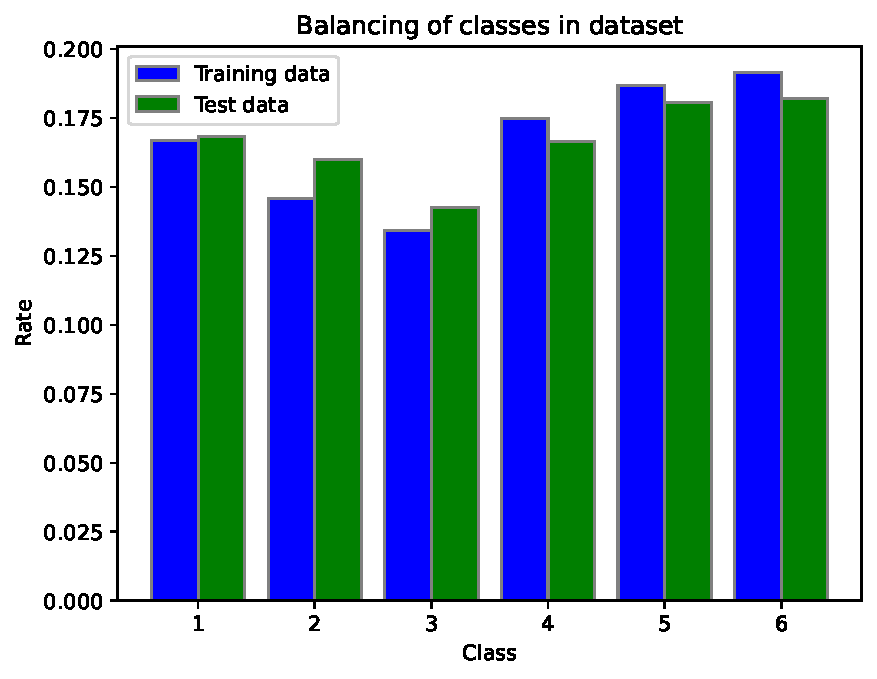
\includegraphics[width=0.6\linewidth]{../../plot/Balancing_of_classes}
	\caption{Gráfico da ocorrência das classes nos conjuntos de dados de treinamento e teste.}
	\label{fig:balancingofclasses}
\end{figure}

\begin{equation}\label{eq:ba}
	BA = \frac{\sum_{i=1}^{Q}Recall_i}{Q} = \frac{\sum_{i=1}^{Q}\frac{\text{TP}_i}{N_i}}{Q} = \frac{\sum_{i=1}^{Q}\frac{\text{TP}_i}{N\cdot Rate_i}}{Q}
\end{equation}



%%%%%%%%%%%%%%%%%%%%%%%%%%%%%%%%%%%%%%%%%%%%%%%%%%%%%%%%%%%
\clearpage
\section{Classificação via Regressão Logística}

A classificação multi-classe é feita de forma elegante ao ter um modelo, que dadas $Q$ classes à serem reconhecidas, apresente $Q$ saídas, onde cada saída é a probabilidade da amostra pertencer à classe em questão. Tal implementação se dá por meio da função \textit{softmax}, enunciada em \eqref{eq:softmax}, e a saída é dada pela notação \textit{one-hot encoding}.

\begin{equation}\label{eq:softmax}
	\hat{y}_k (\+x(i)) = \frac{e^{\left(\+\Phi(\+x(i))^T\+w_k\right)}}{\sum_{j}e^{\left(\+\Phi(\+x(i))^T\+w_j\right)}}
\end{equation}

Onde o $\+w_k$ é o vetor de pesos para a classe $k$, e a matriz de pesos $\+W$ é dada por \eqref{eq:W}.

\begin{equation}\label{eq:W}
	\+W = \begin{bmatrix}
		\+w_1 \\
		\+w_2 \\
		\vdots \\
		\+w_Q
	\end{bmatrix}
\end{equation}

Não existe forma fechada para a obtenção dos pesos de $\+W$, logo, o mesmo precisa ser feito de forma iterativa. A métrica utilizada como função de custo para o problema é a entropia cruzada, dada por \eqref{eq:JCE}. O otimização dos pesos se dá pela técnica do gradiente descendente, dado por \eqref{eq:dJCE}.

\begin{equation}\label{eq:JCE}
	J_{CE}(\+W) = -\sum_{i=0}^{N-1}\sum_{k=1}^{Q}y_{i,k}\log\left[\hat{y}_k(\+x(i)\right]
\end{equation}

\begin{equation}\label{eq:dJCE}
	\nabla\+W = \frac{\partial J_{CE}(\+W)}{\partial \+w_k} = \sum_{i=0}^{N-1} \left(y_{i,k} - \hat{y}_k\left(\+x(i)\right)\right)\+\Phi(\+x(i))^T
\end{equation}

A atualização dos pesos é dada por \eqref{eq:wk1}, onde $l$ é a iteração dos pesos.

\begin{equation}\label{eq:wk1}
	\+W[l+1] = \+W[l] - \eta\nabla\+W
\end{equation}

Devido ao tamanho do conjunto de dados, foi proposto o treinamento por \textit{mini-batch}, testadas com tamanhos de 500, 1000 e 2000 amostras, e um passo ($\eta$) de 0,01, que apresentou boa convergência nos testes realizados \textit{a priori}. O processo de validação cruzada para o treinamento do modelo foi feito na forma \textit{holdout}, considerando o conjunto de validação 30\% do \textit{dataset} de treinamento.



%%%%%%%%%%%%%%%%%%%%%%%%%%%%%%%%%%%%%%%%%%%%%%%%%%%%%%%%%%%
\subsection{Dados tratados}

\subsubsection*{\textit{Mini-batch} 500 amostras}

% TODO: \usepackage{graphicx} required
\begin{figure}[H]
	\begin{subfigure}[H]{0.49\textwidth}
		\centering
		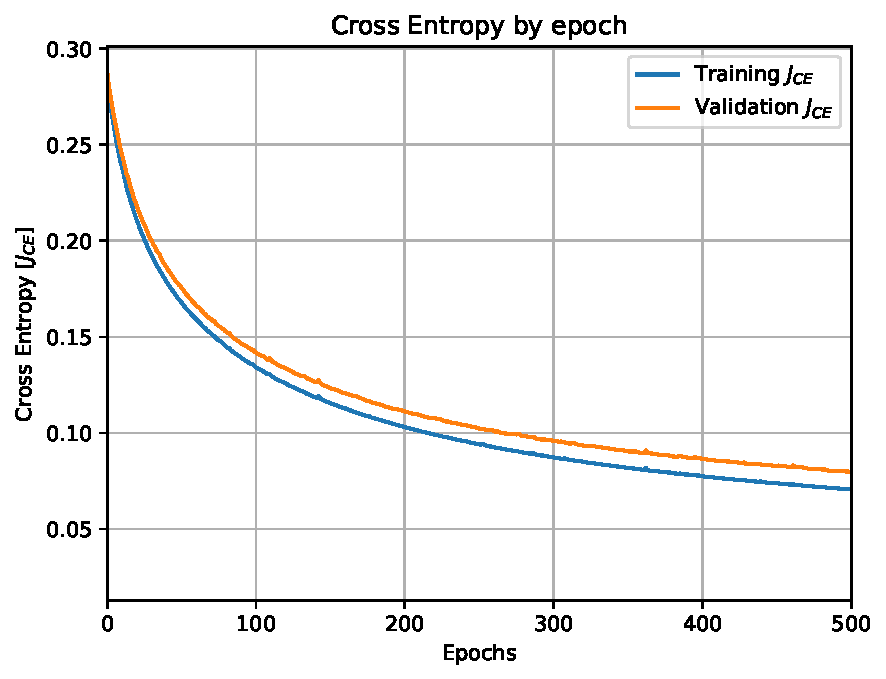
\includegraphics[width = 0.98\linewidth]{../../plot/LR_1/CE_500_epochs_batch_size500}
		\label{fig:CE_500_epochs_batch_size500}
		\caption{Evolução da entropia cruzada.}
	\end{subfigure}
	\begin{subfigure}[H]{0.49\textwidth}
		\centering
		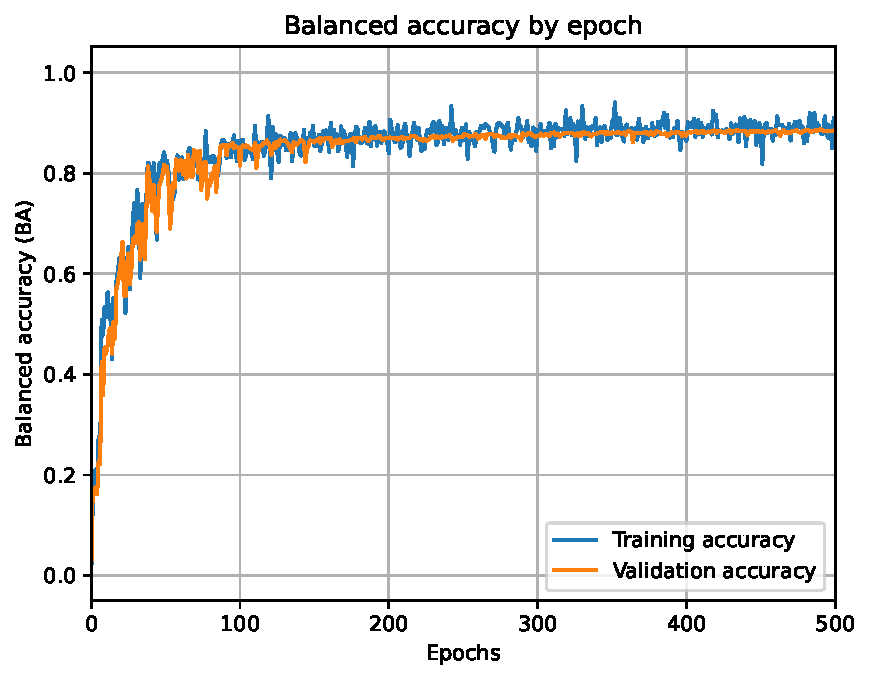
\includegraphics[width = 0.99\linewidth]{../../plot/LR_1/BA_500_epochs_batch_size500}
		\caption{Evolução da acurácia balanceada.}
		\label{fig:BA_500_epochs_batch_size500}
	\end{subfigure}
	\caption{Evolução da entropia cruzada e da acurácia balanceada durante o treinamento para \textit{mini-batch} de 500 amostras e $\eta = 0,01$.}
\end{figure}

\begin{equation}\label{eq:ba_lr_500}
	BA = 0,9162
\end{equation}

\begin{table}[H]
	\centering
\begin{tabular}{c||c|c|c|c|c|c|}
	\cline{2-7}
	& \textbf{1} & \textbf{2} & \textbf{3} & \textbf{4} & \textbf{5} & \textbf{6} \\ \hline \hline
	\multicolumn{1}{|c||}{\textbf{1}} & 486        & 0          & 10         & 0          & 0          & 0          \\ \hline
	\multicolumn{1}{|c||}{\textbf{2}} & 30         & 440        & 1          & 0          & 0          & 0          \\ \hline
	\multicolumn{1}{|c||}{\textbf{3}} & 39         & 52         & 329        & 0          & 0          & 0          \\ \hline
	\multicolumn{1}{|c||}{\textbf{4}} & 0          & 3          & 0          & 424        & 64         & 0          \\ \hline
	\multicolumn{1}{|c||}{\textbf{5}} & 1          & 0          & 0          & 33         & 498        & 0          \\ \hline
	\multicolumn{1}{|c||}{\textbf{6}} & 0          & 0          & 0          & 0          & 0          & 537        \\ \hline
\end{tabular}
	\caption{Matriz de confusão do classificador com \textit{mini-batch} de 500 amostras.}
	\label{tab:mc_lr_500}
\end{table}

\begin{table}[H]
	\centering
	\begin{tabular}{c|c|c}
		\textbf{Classe} & \textbf{Precisão} & \textit{\textbf{Recall}} \\ \hline
		\textbf{1}      & 0.9798            & 0.8741                   \\
		\textbf{2}      & 0.9342            & 0.8889                   \\
		\textbf{3}      & 0.7833            & 0.9676                   \\
		\textbf{4}      & 0.8635            & 0.9278                   \\
		\textbf{5}      & 0.9361            & 0.8861                   \\
		\textbf{6}      & 1.0000            & 1.0000                  
	\end{tabular}
	\caption{Precisão e \textit{Recall} do classificador com \textit{mini-batch} de 500 amostras por classe.}
	\label{tab:pr_lr_500}
\end{table}



\subsubsection*{\textit{Mini-batch} 1000 amostras}

% TODO: \usepackage{graphicx} required
\begin{figure}[H]
	\begin{subfigure}[H]{0.49\textwidth}
		\centering
		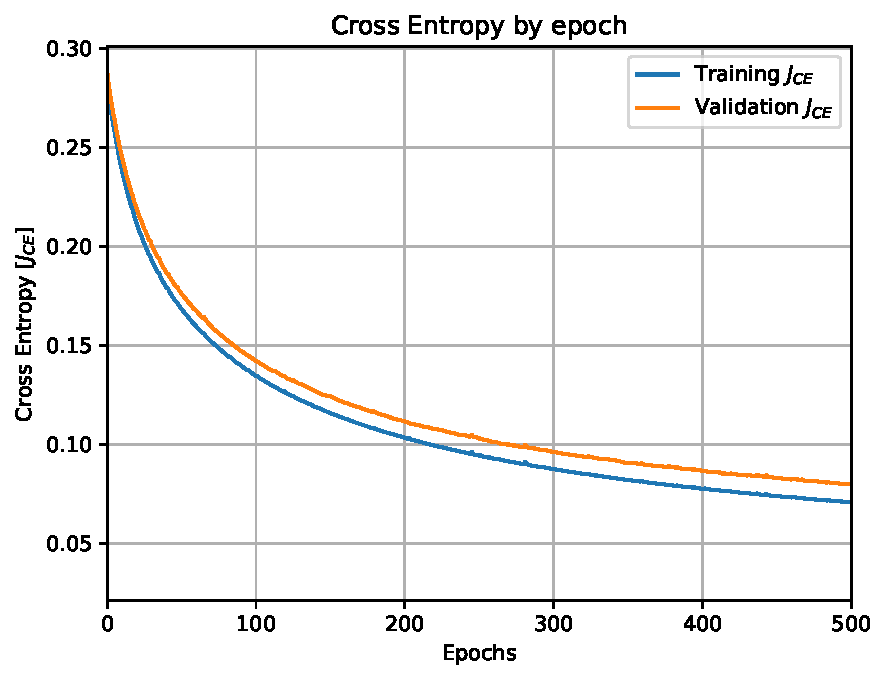
\includegraphics[width = 0.98\linewidth]{../../plot/LR_1/CE_500_epochs_batch_size1000}
		\label{fig:CE_500_epochs_batch_size1000}
		\caption{Evolução da entropia cruzada.}
	\end{subfigure}
	\begin{subfigure}[H]{0.49\textwidth}
		\centering
		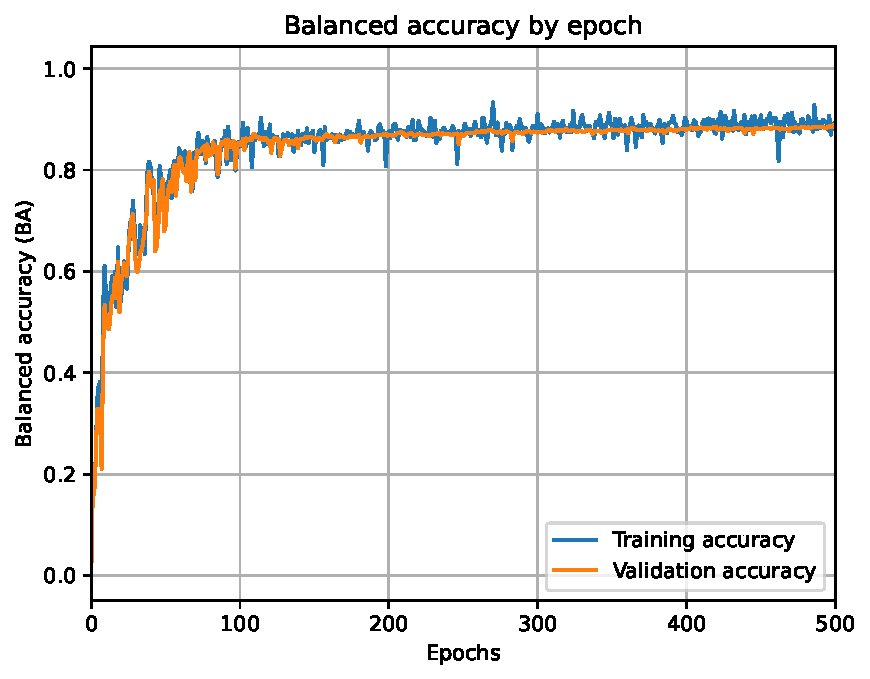
\includegraphics[width = 0.99\linewidth]{../../plot/LR_1/BA_500_epochs_batch_size1000}
		\caption{Evolução da acurácia balanceada.}
		\label{fig:BA_500_epochs_batch_size1000}
	\end{subfigure}
	\caption{Evolução da entropia cruzada e da acurácia balanceada durante o treinamento para \textit{mini-batch} de 1000 amostras e $\eta = 0,01$.}
\end{figure}

\begin{equation}\label{eq:ba_lr_1000}
BA = 0,9042
\end{equation}

\begin{table}[H]
\centering
\begin{tabular}{c||c|c|c|c|c|c|}
	\cline{2-7}
	& \textbf{1} & \textbf{2} & \textbf{3} & \textbf{4} & \textbf{5} & \textbf{6} \\ \hline\hline
	\multicolumn{1}{|c||}{\textbf{1}} & 486        & 0          & 10         & 0          & 0          & 0          \\ \hline
	\multicolumn{1}{|c||}{\textbf{2}} & 28         & 443        & 0          & 0          & 0          & 0          \\ \hline
	\multicolumn{1}{|c||}{\textbf{3}} & 56         & 53         & 311        & 0          & 0          & 0          \\ \hline
	\multicolumn{1}{|c||}{\textbf{4}} & 0          & 3          & 0          & 426        & 61         & 1          \\ \hline
	\multicolumn{1}{|c||}{\textbf{5}} & 0          & 1          & 0          & 54         & 477        & 0          \\ \hline
	\multicolumn{1}{|c||}{\textbf{6}} & 0          & 0          & 0          & 0          & 0          & 537        \\ \hline
\end{tabular}
\caption{Matriz de confusão do classificador com \textit{mini-batch} de 1000 amostras.}
\label{tab:mc_lr_1000}
\end{table}

\begin{table}[H]
\centering
\begin{tabular}{c|c|c}
	\textbf{Classe} & \textbf{Precisão} & \textit{\textbf{Recall}} \\ \hline
	\textbf{1}      & 0.9798            & 0.8526                   \\
	\textbf{2}      & 0.9406            & 0.8860                   \\
	\textbf{3}      & 0.7405            & 0.9688                   \\
	\textbf{4}      & 0.8676            & 0.8875                   \\
	\textbf{5}      & 0.8966            & 0.8866                   \\
	\textbf{6}      & 1.0000            & 0.9981                  
\end{tabular}
\caption{Precisão e \textit{Recall} do classificador com \textit{mini-batch} de 1000 amostras por classe.}
\label{tab:pr_lr_1000}
\end{table}







\subsubsection*{\textit{Mini-batch} 2000 amostras}

% TODO: \usepackage{graphicx} required
\begin{figure}[H]
	\begin{subfigure}[H]{0.49\textwidth}
		\centering
		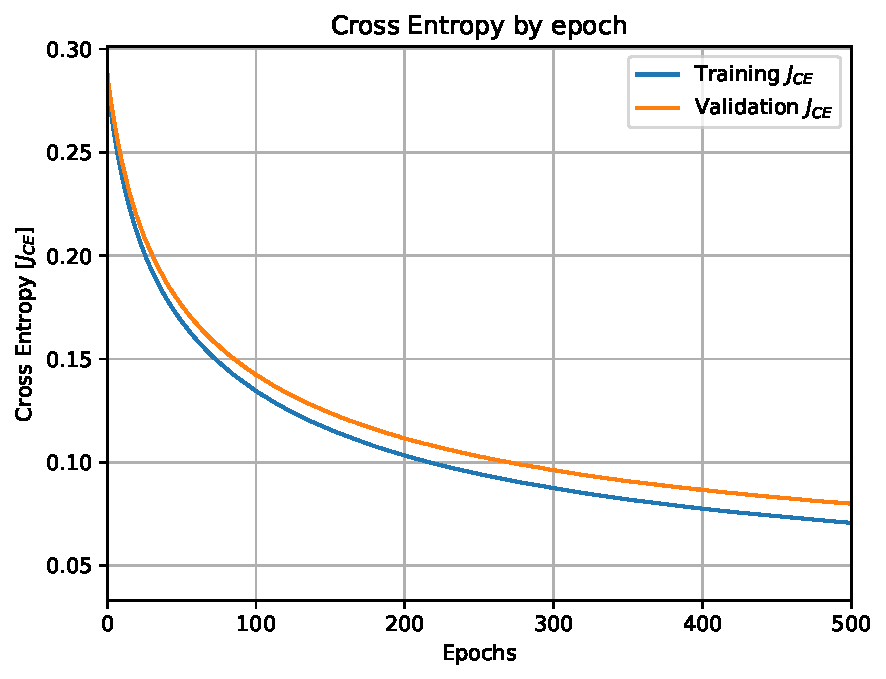
\includegraphics[width = 0.98\linewidth]{../../plot/LR_1/CE_500_epochs_batch_size2000}
		\label{fig:CE_500_epochs_batch_size2000}
		\caption{Evolução da entropia cruzada.}
	\end{subfigure}
	\begin{subfigure}[H]{0.49\textwidth}
		\centering
		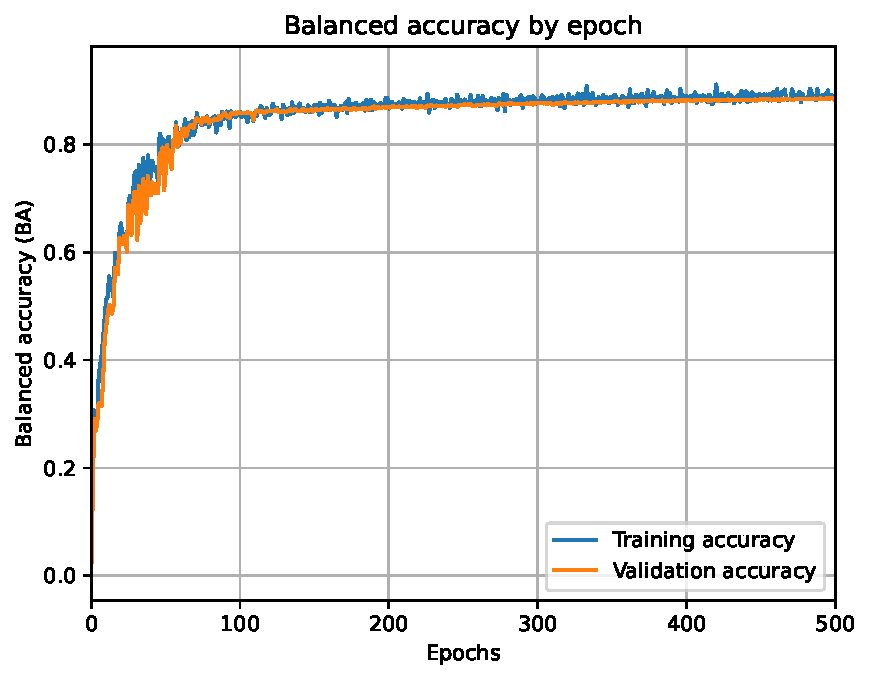
\includegraphics[width = 0.99\linewidth]{../../plot/LR_1/BA_500_epochs_batch_size2000}
		\caption{Evolução da acurácia balanceada.}
		\label{fig:BA_500_epochs_batch_size2000}
	\end{subfigure}
	\caption{Evolução da entropia cruzada e da acurácia balanceada durante o treinamento para \textit{mini-batch} de 2000 amostras e $\eta = 0,01$.}
\end{figure}

\begin{equation}\label{eq:ba_lr_2000}
BA = 0,8898
\end{equation}

\begin{table}[H]
\centering
\begin{tabular}{c|c|c|c|c|c|c|}
	\cline{2-7}
	& \textbf{1} & \textbf{2} & \textbf{3} & \textbf{4} & \textbf{5} & \textbf{6} \\ \hline\hline
	\multicolumn{1}{|c||}{\textbf{1}} & 489        & 0          & 7          & 0          & 0          & 0          \\ \hline
	\multicolumn{1}{|c||}{\textbf{2}} & 27         & 444        & 0          & 0          & 0          & 0          \\ \hline
	\multicolumn{1}{|c||}{\textbf{3}} & 70         & 49         & 301        & 0          & 0          & 0          \\ \hline
	\multicolumn{1}{|c||}{\textbf{4}} & 0          & 3          & 0          & 396        & 91         & 1          \\ \hline
	\multicolumn{1}{|c||}{\textbf{5}} & 1          & 1          & 0          & 58         & 472        & 0          \\ \hline
	\multicolumn{1}{|c||}{\textbf{6}} & 0          & 0          & 0          & 0          & 0          & 537        \\ \hline
\end{tabular}
\caption{Matriz de confusão do classificador com \textit{mini-batch} de 2000 amostras.}
\label{tab:mc_lr_2000}
\end{table}

\begin{table}[H]
\centering
\begin{tabular}{c|c|c}
	\textbf{Classe} & \textbf{Precisão} & \textit{\textbf{Recall}} \\ \hline
	\textbf{1}      & 0.9859            & 0.8330                   \\
	\textbf{2}      & 0.9427            & 0.8934                   \\
	\textbf{3}      & 0.7167            & 0.9773                   \\
	\textbf{4}      & 0.8065            & 0.8722                   \\
	\textbf{5}      & 0.8872            & 0.8384                   \\
	\textbf{6}      & 1.0000            & 0.9981                  
\end{tabular}
\caption{Precisão e \textit{Recall} do classificador com \textit{mini-batch} de 2000 amostras por classe.}
\label{tab:pr_lr_2000}
\end{table}

\subsubsection*{Análise}

\begin{figure}[H]
	\begin{subfigure}[H]{0.49\textwidth}
		\centering
		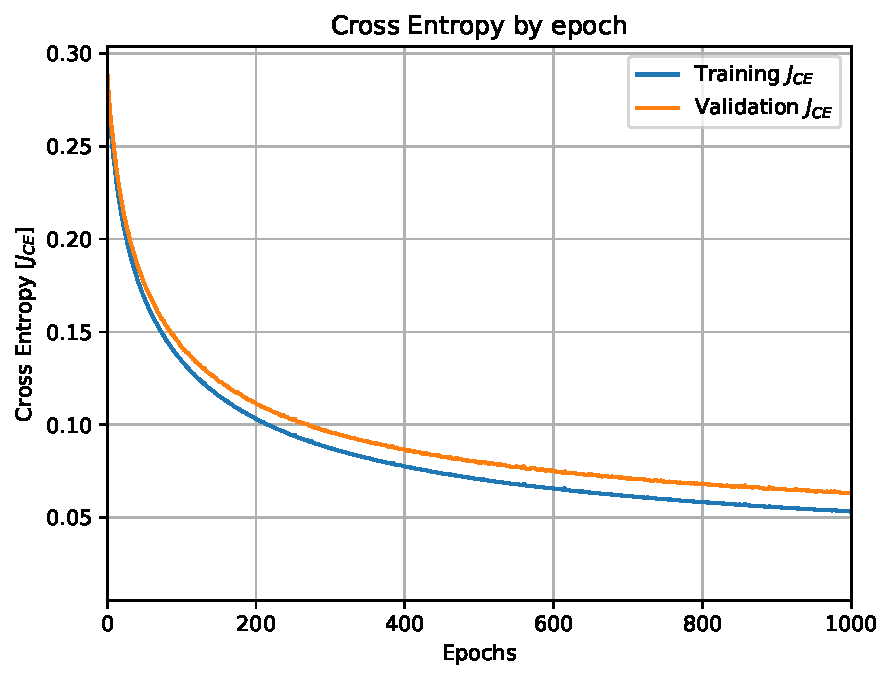
\includegraphics[width = 0.98\linewidth]{../../plot/LR_1/CE_1000_epochs_batch_size500}
		\label{fig:CE_1000_epochs_batch_size500}
		\caption{Evolução da entropia cruzada.}
	\end{subfigure}
	\begin{subfigure}[H]{0.49\textwidth}
		\centering
		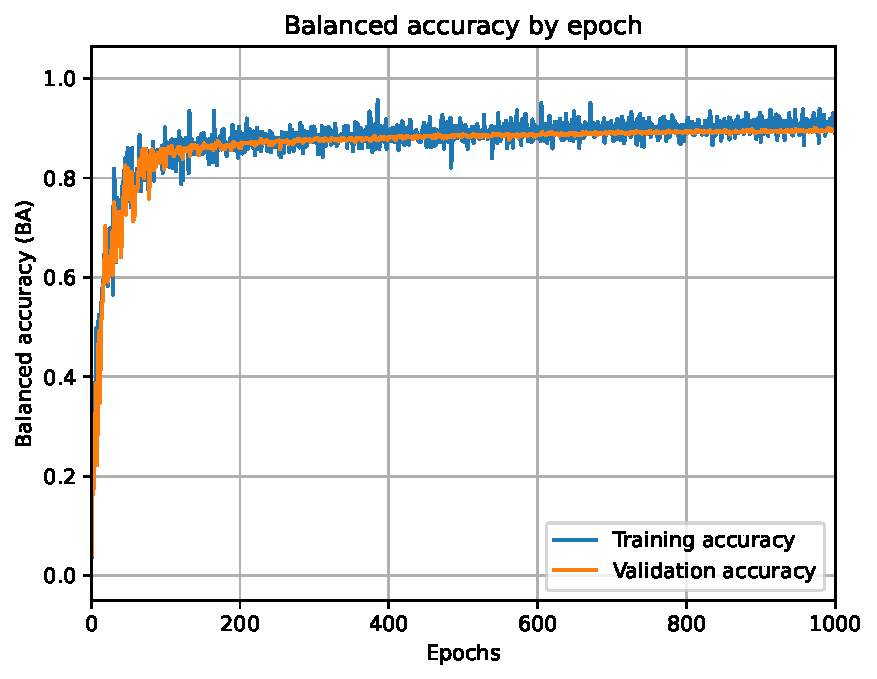
\includegraphics[width = 0.99\linewidth]{../../plot/LR_1/BA_1000_epochs_batch_size500}
		\caption{Evolução da acurácia balanceada.}
		\label{fig:BA_1000_epochs_batch_size500}
	\end{subfigure}
	\caption{Entropia cruzada e acurácia balanceada para o treinamento do modelo com \textit{mini-batch} de 500 amostras por 1000 épocas.}
\end{figure}





%%%%%%%%%%%%%%%%%%%%%%%%%%%%%%%%%%%%%%%%%%%%%%%%%%%%%%%%%%%
\subsection{Dados brutos}







%%%%%%%%%%%%%%%%%%%%%%%%%%%%%%%%%%%%%%%%%%%%%%%%%%%%%%%%%%%
\clearpage
\section{Classificação via \textit{k neareast neighbours}}

A classificação pelo método \textit{k neareast neighbours} é baseada em inferir a classe do dado a ser classificado com base nos $k$ dados mais próximos à ele. Como hiper-parâmetros para esse problema, têm-se principalmente o valor de $k$, a ordem $p$ da distância de Minkowski entre os dados e o critério de classificação.

O critério de classificação pode se basear puramente na classe majoritária entre os $k$ vizinhos, ou levar em consideração a distância como um peso, que normalmente é inversamente proporcional a distância, evidenciando o rótulo dos pontos mais próximos do dado teste.


%%%%%%%%%%%%%%%%%%%%%%%%%%%%%%%%%%%%%%%%%%%%%%%%%%%%%%%%%%%
\subsection{Dados tratados}

Para implementação do algoritmo de \textit{k}NN, foi escolhido a utilização da distância euclidiana no espaço dos atributos, e a decisão do rótulo vencedor por meio do voto majoritário dos $k$ vizinhos mais próximos.

Para obtenção do valor de $k$, foi executada uma busca em \textit{grid} do hiper-parâmetro, variando seu valor entre 1 e 29. Utilizando da técnica de validação cruzada \textit{k-fold}, com quatro pastas, foi realizada a inferência das classes dos dados da pasta de validação com base nos vizinhos mais próximos encontrados nas pastas de treinamento, para cada valor de $k$ testado. A \autoref{fig:gridsearch} exibe à evolução da acurácia balanceada para os valores de $k$, obtendo um conjunto de valores ótimos em \eqref{eq:k_fold_k}.

\begin{equation}\label{eq:k_fold_k}
	k = [17\ 28\ 12\ 18]
\end{equation}


% TODO: \usepackage{graphicx} required
\begin{figure}[H]
	\centering
	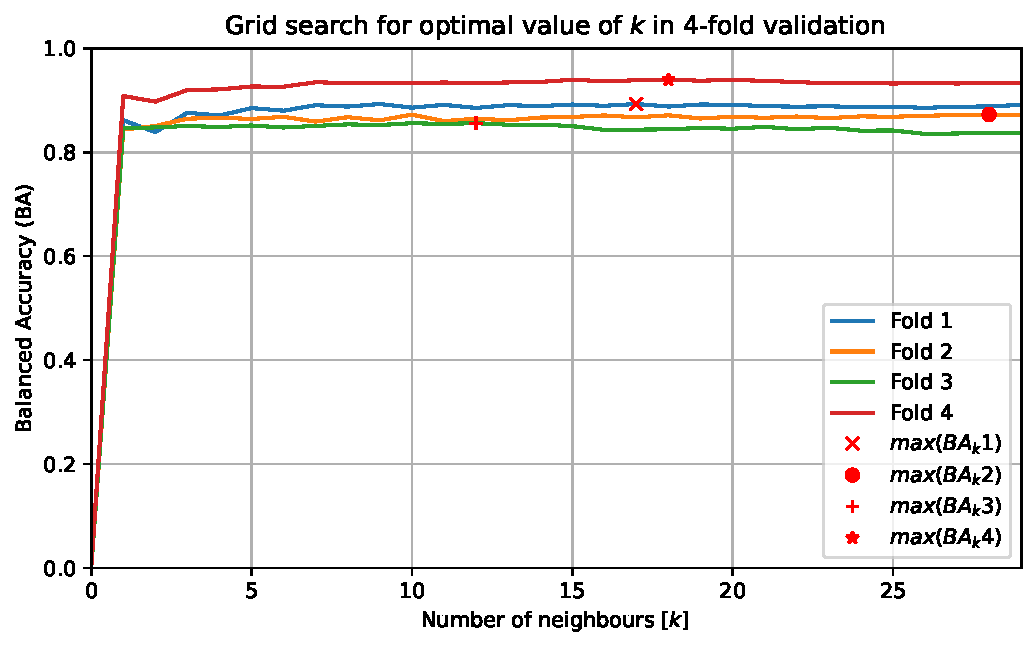
\includegraphics[width=0.75\linewidth]{../../plot/knn_1/grid_search_k_fold}
	\caption{Busca em \textit{grid} do valor de $k$ ótimo utilizando \textit{4-fold validation}.}
	\label{fig:gridsearch}
\end{figure}

A heurística escolhida para avaliar o melhor valor de $k$ com base no conjunto obtido por meio da busca em \textit{grid} com validação cruzada se dá em obter a acurácia balanceada média das pastas e obter o número de vizinhos que maximiza essa combinação das pastas. A \autoref{fig:gridsearch-k_optimal} mostra a progressão da acurácia balanceada média de acordo com $k$, e assim se obtém o valor de $k$ ótimo em $k = 15$.

\begin{figure}[H]
	\centering
	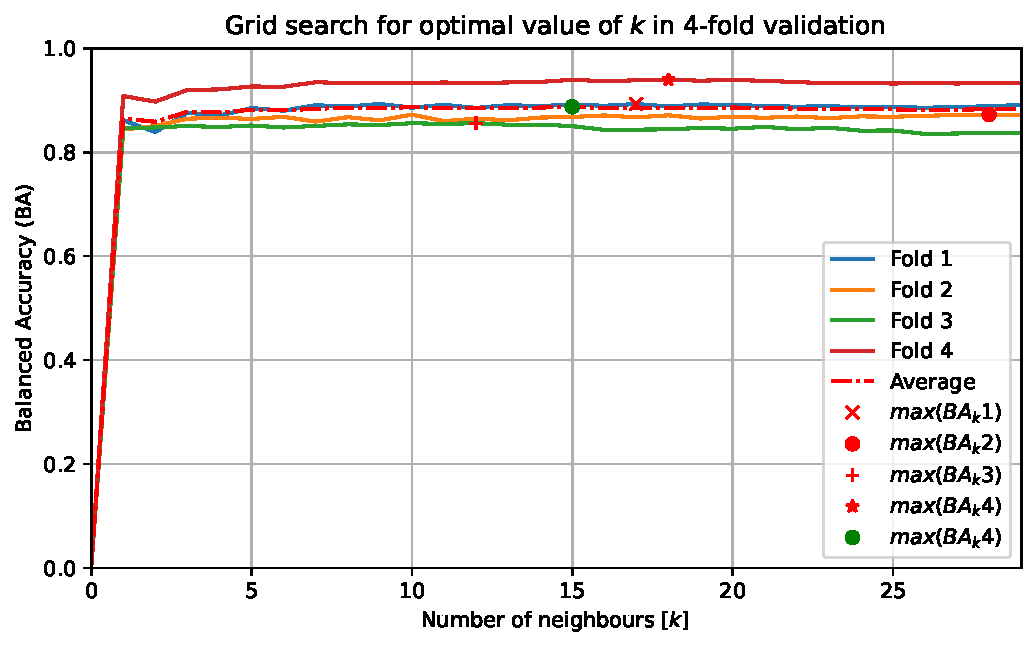
\includegraphics[width=0.75\linewidth]{../../plot/knn_1/grid_search_k_fold-k_optimal}
	\caption{Busca em \textit{grid} do valor de $k$ ótimo utilizando \textit{4-fold validation}.}
	\label{fig:gridsearch-k_optimal}
\end{figure}



Uma vez definido o classificador ótimo, obtém-se os indicadores de performance do classificador com base nos dados de teste. A acurácia balanceada encontrada foi de 0,8991 e a matriz de confusão do classificador por ser vista na \autoref{tab:mc_knn_1}.

\begin{equation}\label{eq:ba_knn_1}
	BA = 0,8991
\end{equation}

\begin{table}[H]
	\centering
	\begin{tabular}{c||c|c|c|c|c|c|}
		\cline{2-7}
		& \textbf{1} & \textbf{2} & \textbf{3} & \textbf{4} & \textbf{5} & \multicolumn{1}{l|}{\textbf{6}} \\ \hline \hline
		\multicolumn{1}{|c||}{\textbf{1}} & 488 & 0   & 8   & 0   & 0   & 0   \\ \hline
		\multicolumn{1}{|c||}{\textbf{2}} & 39  & 427 & 5   & 0   & 0   & 0   \\ \hline
		\multicolumn{1}{|c||}{\textbf{3}} & 51  & 44  & 325 & 0   & 0   & 0   \\ \hline
		\multicolumn{1}{|c||}{\textbf{4}} & 0   & 4   & 0   & 389 & 98  & 0   \\ \hline
		\multicolumn{1}{|c||}{\textbf{5}} & 0   & 0   & 0   & 31  & 501 & 0   \\ \hline
		\multicolumn{1}{|c||}{\textbf{6}} & 0   & 0   & 0   & 1   & 1   & 535 \\ \hline
	\end{tabular}
	\caption{Matriz de confusão do classificador k-NN com k = 15.}
	\label{tab:mc_knn_1}
\end{table}

Extraindo da matriz de confusão as métricas de precisão e \textit{recall}, obtém-se a \autoref{tab:pr_knn_1}. Pode-se observar que a classe 3 foi a que apresentou menor precisão, sendo muito confundida com a classe 1 e 2. Já a classe 1 possuí o pior \textit{recall}, uma vez que as classes 2 e 3 se confundem com a 1. A classe 6 foi a que apresentou o melhor desempenho, apresentando \textit{recall} unitário, logo, nenhuma classe se confunde com ela, e a maior precisão, muito próxima de 1.


\begin{table}[H]
	\centering
	\begin{tabular}{c|c|c}
		\textbf{Classe} & \textbf{Precisão} & \textbf{\textit{Recall}} \\ \hline
		\textbf{1}      & 0.9839 & 0.8443 \\
		\textbf{2}      & 0.9066 & 0.8989 \\
		\textbf{3}      & 0.7738 & 0.9615 \\
		\textbf{4}      & 0.7923 & 0.9240 \\
		\textbf{5}      & 0.9417 & 0.8350 \\
		\textbf{6}      & 0.9963 & 1.0000
	\end{tabular}
	\caption{Precisão e \textit{Recall} do classificador por classe.}
	\label{tab:pr_knn_1}
\end{table}

\subsubsection*{Comparação com a regressão logística}

Ao comparar os classificadores utilizando a regressão logística e o k-NN, observa-se que a acurácia balanceada para a regressão logística de melhor desempenho foi superior, mas para ter uma comparação mais minuciosa entre os dois classificadores, deve-se analisar também suas matrizes de confusão. Comparando a precisão e o \textit{recall}, o desempenho das classes em \textit{ranking} se apresenta da mesma forma, porém, para a regressão logística a classe 6 conseguiu obter tanto precisão quanto \textit{recall} máximo.

A regressão logística apresentou um desempenho 1,87\% maior que o k-NN para a acurácia balanceada, porém possuí uma complexidade muito maior. Para obter o modelo de regressão logística multi-classe com \textit{softmax}, é necessário realizar o treinamento do modelo, buscando variar os hiper-parâmetros para se conseguir o melhor desempenho. Essa etapa demanda de muito processamento, porém garante uma utilização do classificador mais leve, uma vez que é necessária apenas o vetor de pesos. Já o k-NN, não demanda treinamento, sendo necessária apenas a inferência da classe com base nos vizinhos mais próximos, o que apesar de consumir armazenamento para manter o \textit{dataset}, não precisa de tanto processamento prévio, sendo uma solução simples e rápida. Porém, devido a busca em \textit{grid} utilizando a validação \textit{k-fold} para obter o melhor $k$ para os dados de treinamento, tal etapa demandou bastante processamento, o que elevou consideravelmente a complexidade do k-NN.


%%%%%%%%%%%%%%%%%%%%%%%%%%%%%%%%%%%%%%%%%%%%%%%%%%%%%%%%%%%
\subsection{Dados brutos}







%%%%%%%%%%%%%%%%%%%%%%%%%%%%%%%%%%%%%%%%%%%%%%%%%%%%%%%%%%%
\section{Comparação entre os classificadores}

\subsection{Dados tratados}


